% !TEX TS-program = xelatex
% !TeX spellcheck = ru_RU
% !TEX root = sel1.tex

\documentclass[tikz,border=3.14mm]{standalone}

\usepackage{tikz}
\usetikzlibrary{graphs, positioning}

\def\mynode#1#2 {
      \node[box] (b#1) {#2};
      \node [right,inner xsep=.5em
          , outer sep=0pt,text height=1ex,text depth=.0ex] (caption#1)
                   at ([shift={(-1em,0pt)}]b#1.north west) {#1};
}

\begin{document}
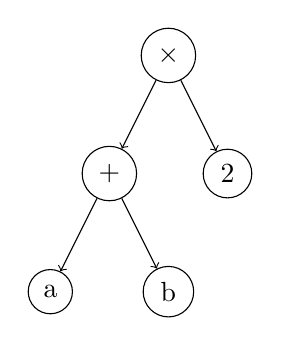
\begin{tikzpicture}[nodes={draw, circle}, ->]
\node{$\times$}
child { node {+}
    child { node {a} }
    child { node {b} }
}
child { node {2} };
\end{tikzpicture}


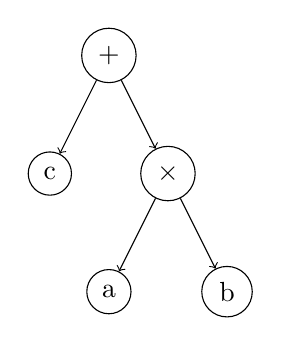
\begin{tikzpicture}[nodes={draw, circle}, ->]
    \node{+}
    child { node {c} }
    child { node {$\times$}
        child { node {a} }
        child { node {b} }
    };
\end{tikzpicture}



\tikzset{
    op/.style={draw, circle},
    rand/.style={draw, circle},
    lab/.style={}
}

\begin{tikzpicture}
\draw[help lines,step=5mm,gray!20] (-4,-4) grid (4,3);
\node[op] (t1) at (0,0) { = };
\node[rand,above left=of t1] () { 0 };
\node[op,above right=of t1] (c3) { {\tiny mod} };
\node[op,above left=of c3] (c0) { 2 };


\draw[red] (c3) to [bend right=10] (t1);

    %    \begin{scope}[yshift=8cm,node distance=2cm and 1cm]
        %        \draw[help lines,step=5mm,gray!20] (-4,-4) grid (4,3);
        %        \node[draw] (a) at (0,0) {a};
        %        \foreach \pos in {above,above right,right,below right,below,below left,left,above left}
        %        \node[draw,\pos = of a] () {\pos};
        %    \end{scope}
\end{tikzpicture}

\end{document}